\section*{سوال ۶}

تحلیل روش طراحی ویژگی‌رانه (نسخه سوم) را به دقت مطالعه کنید و تحلیل خود را از این روش براساس موارد زیر بیان کنید.

\section*{مستندات معماری}
شامل تصمیمات، عقلانیت، دیدگاه‌های معماری، راه‌حل‌های جایگزین، بازنمایی و سایر موارد اشاره شده در کتاب.

\section*{نگرانی‌های همه انواع ذی‌نفعان}
شامل کاربر نهایی، مشتری، تیم ایجاد، مدیر پروژه و …

\section*{چگونگی کاربرد مفاهیم، اصول، الگوها و سبک‌های معماری}
بررسی نحوه کاربرد این مفاهیم در روش طراحی ویژگی رانه.

توجه کنید پوشایی و دقت پاسخ شما به عنوان ملاک مهم ارزیابی در این سوال در نظر گرفته می‌شود.

\section*{جواب سوال ۶}

\begin{figure}[H]
	\centering
	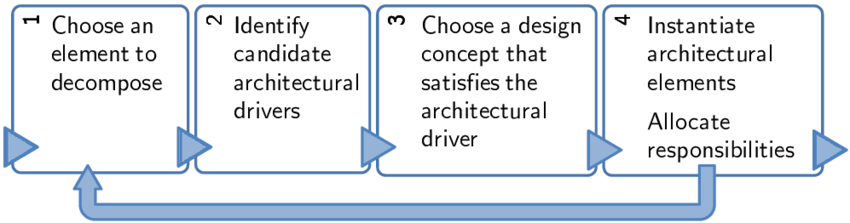
\includegraphics{pic10.png}
	\label{fig:label4}
\end{figure}

\begin{figure}[H]
	\centering
	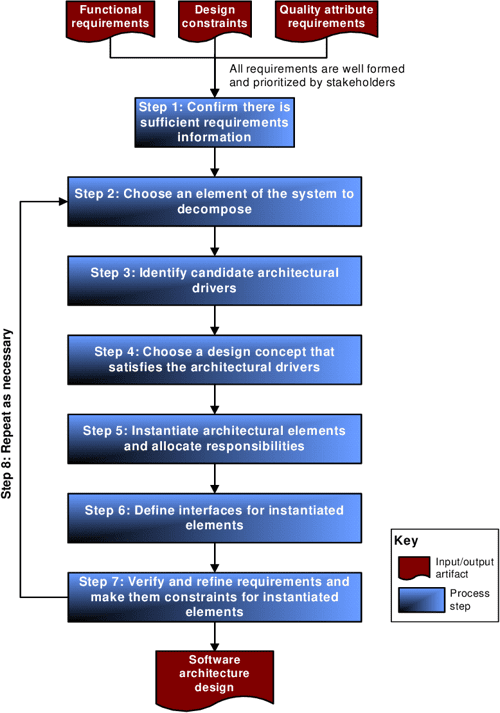
\includegraphics{pic11.png}
	\label{fig:label4}
\end{figure}